
\section{Optimierung des ARM}
In diesem Kapitel werden die Optimierungen am Code beschrieben, der rein auf dem ARM Cortex-A8 ausgef�hrt wird. Hierf�r werden die in \textbf{Kapitel \ref{subsec:a8}} beschriebenen Hardwareemelemte ausgenutzt.\\
In \textbf{Abschnitt \ref{subsec:armtime}} wird daher als erstes die Laufzeitmessung des gesamten Programms (Extraktion, Prozessierung und Klassifikation) erl�utert, um einen Einstiegspunkt f�r die Optimierung zu extrahieren. In den darauffolgenden Abschnitten werden daraufhin die durchgef�hrten Optimierungen beschrieben. 

\subsection{Laufzeitmessung des Gesamtprogramms}\label{subsec:armtime}
F�r die erste Laufzeitmessung des gesammten Programms (Extraktion, Prozessierung und Klassifikation) wurde dieses mit den in \textbf{Kapitel \ref{ph:neoncomp}} beschriebenen Compileroptionen zur automatischen Generierung von NEON-Code kompiliert. Die dabei resultierten Laufzeiten sind in \textbf{Abbildung \ref{fig:mclneon}} abzulesen.
%
\begin{figure}[htp]
	\centering
		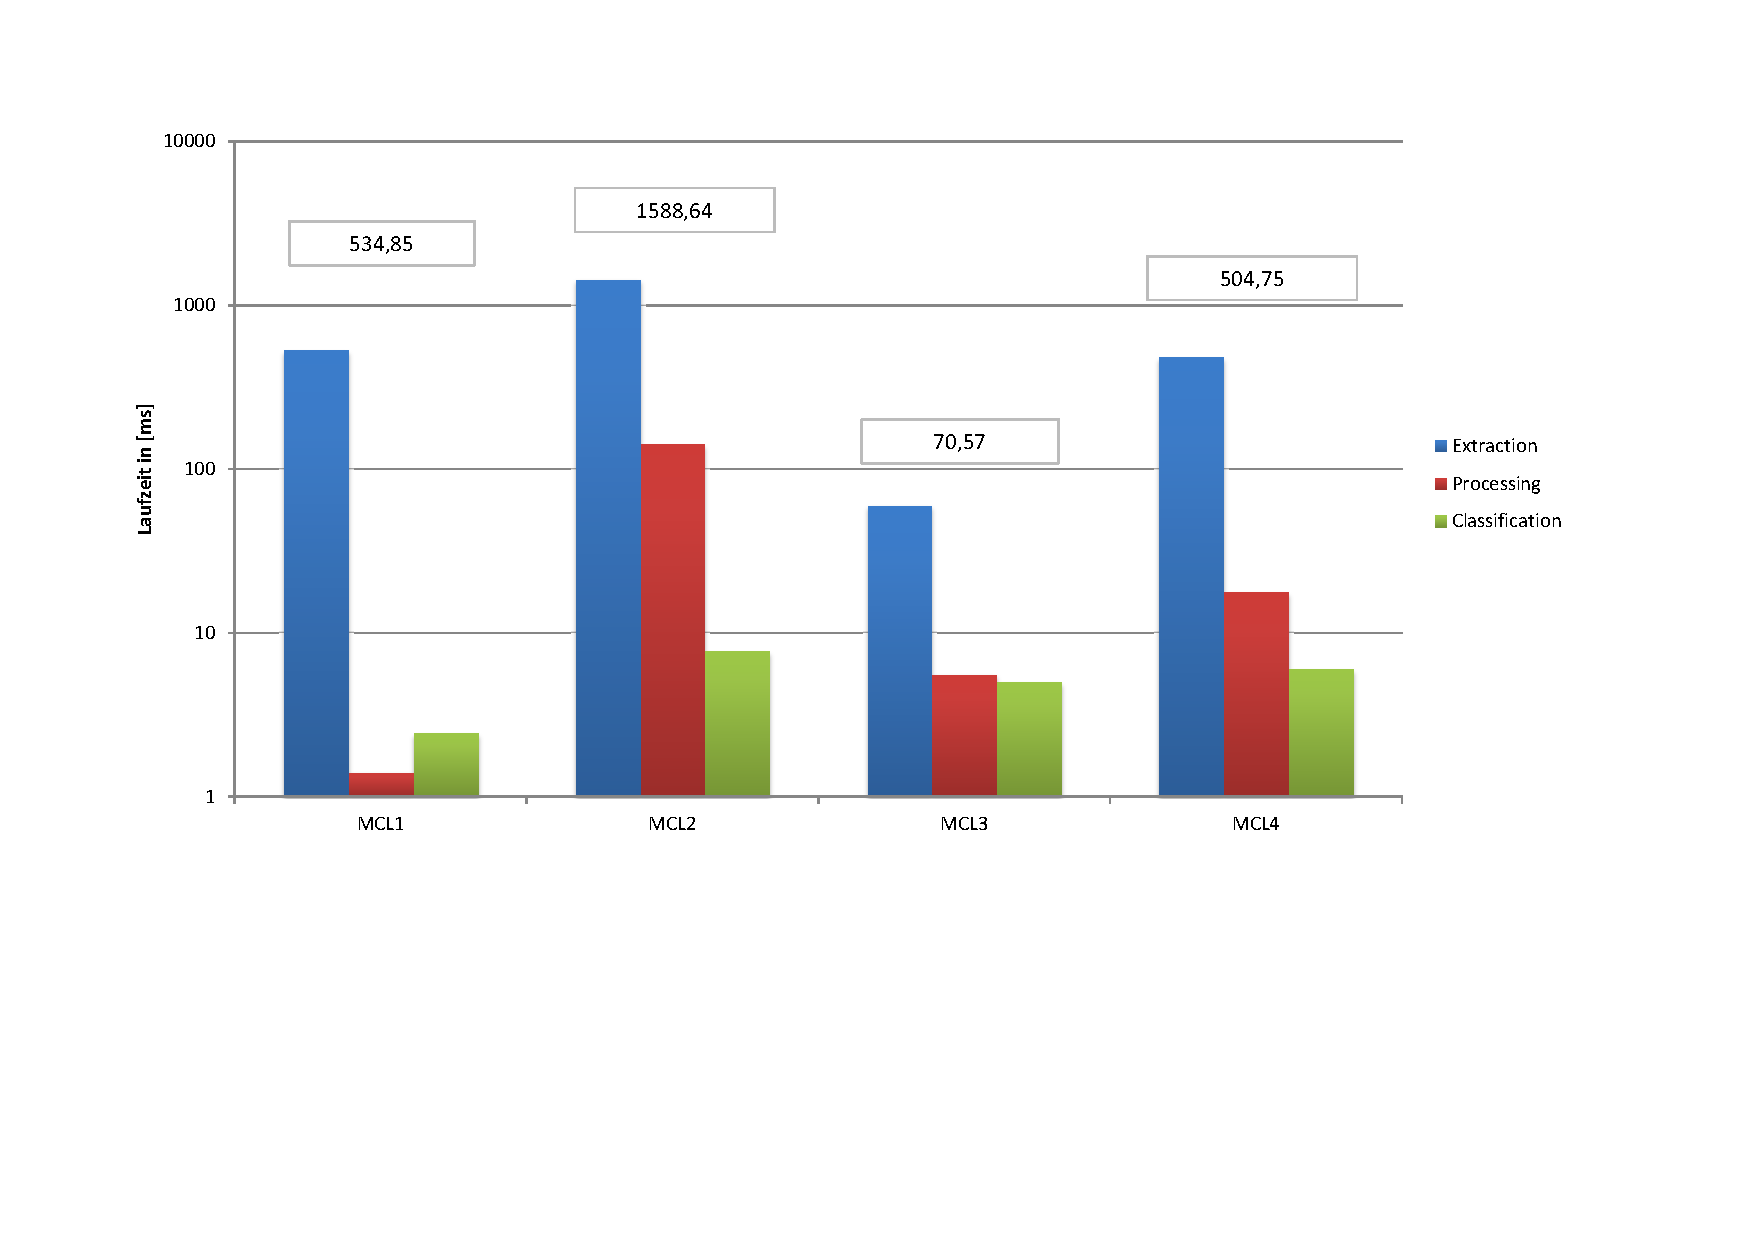
\includegraphics[width=1\textwidth]{../Pictures/mclneon.pdf}
	\caption{Laufzeiten in ms des Musikklassifikators}
	\label{fig:mclneon}
\end{figure} 
%
Wie man aus der Abbildung entnehmen kann, f�llt der gr��te Anteil an der Gesamtlaufzeit in allen vier Messungen (\textit{MCL1 - MCL4}) auf die Extraktionsphase. Hierbei stellt sich jetzt allerdings die Frage, ob das nur an der Komibation aus ARM und NEON liegt oder ob dieses eine generelle Tendenz ist. Darum muss die Laufzeitmessung der genannten Komibation noch mit den Laufzeitmessungen von einer reinen ARM-Implementation und der Kombination aus ARM und VFP-Einheit (vgl. \textbf{Kapitel \ref{ph:vfp}}) verglichen werden. Die Ergebnisse dieser sind in \textbf{Abbildung \ref{fig:armtime}} abzulesen. Diese und alle weiteren Messungen werden am Beispiel des in \textbf{Kapitel \ref{subsec:fset2}} beschriebenen FeatureSets durchgef�hrt, die Diagramme f�r die anderen drei FeatureSets sind f�r den interessierten Leser im Anhang zu finden, aber f�r diese sind die beschriebenen Tatsachen equivalent.
%
\begin{figure}[h]
	\centering
		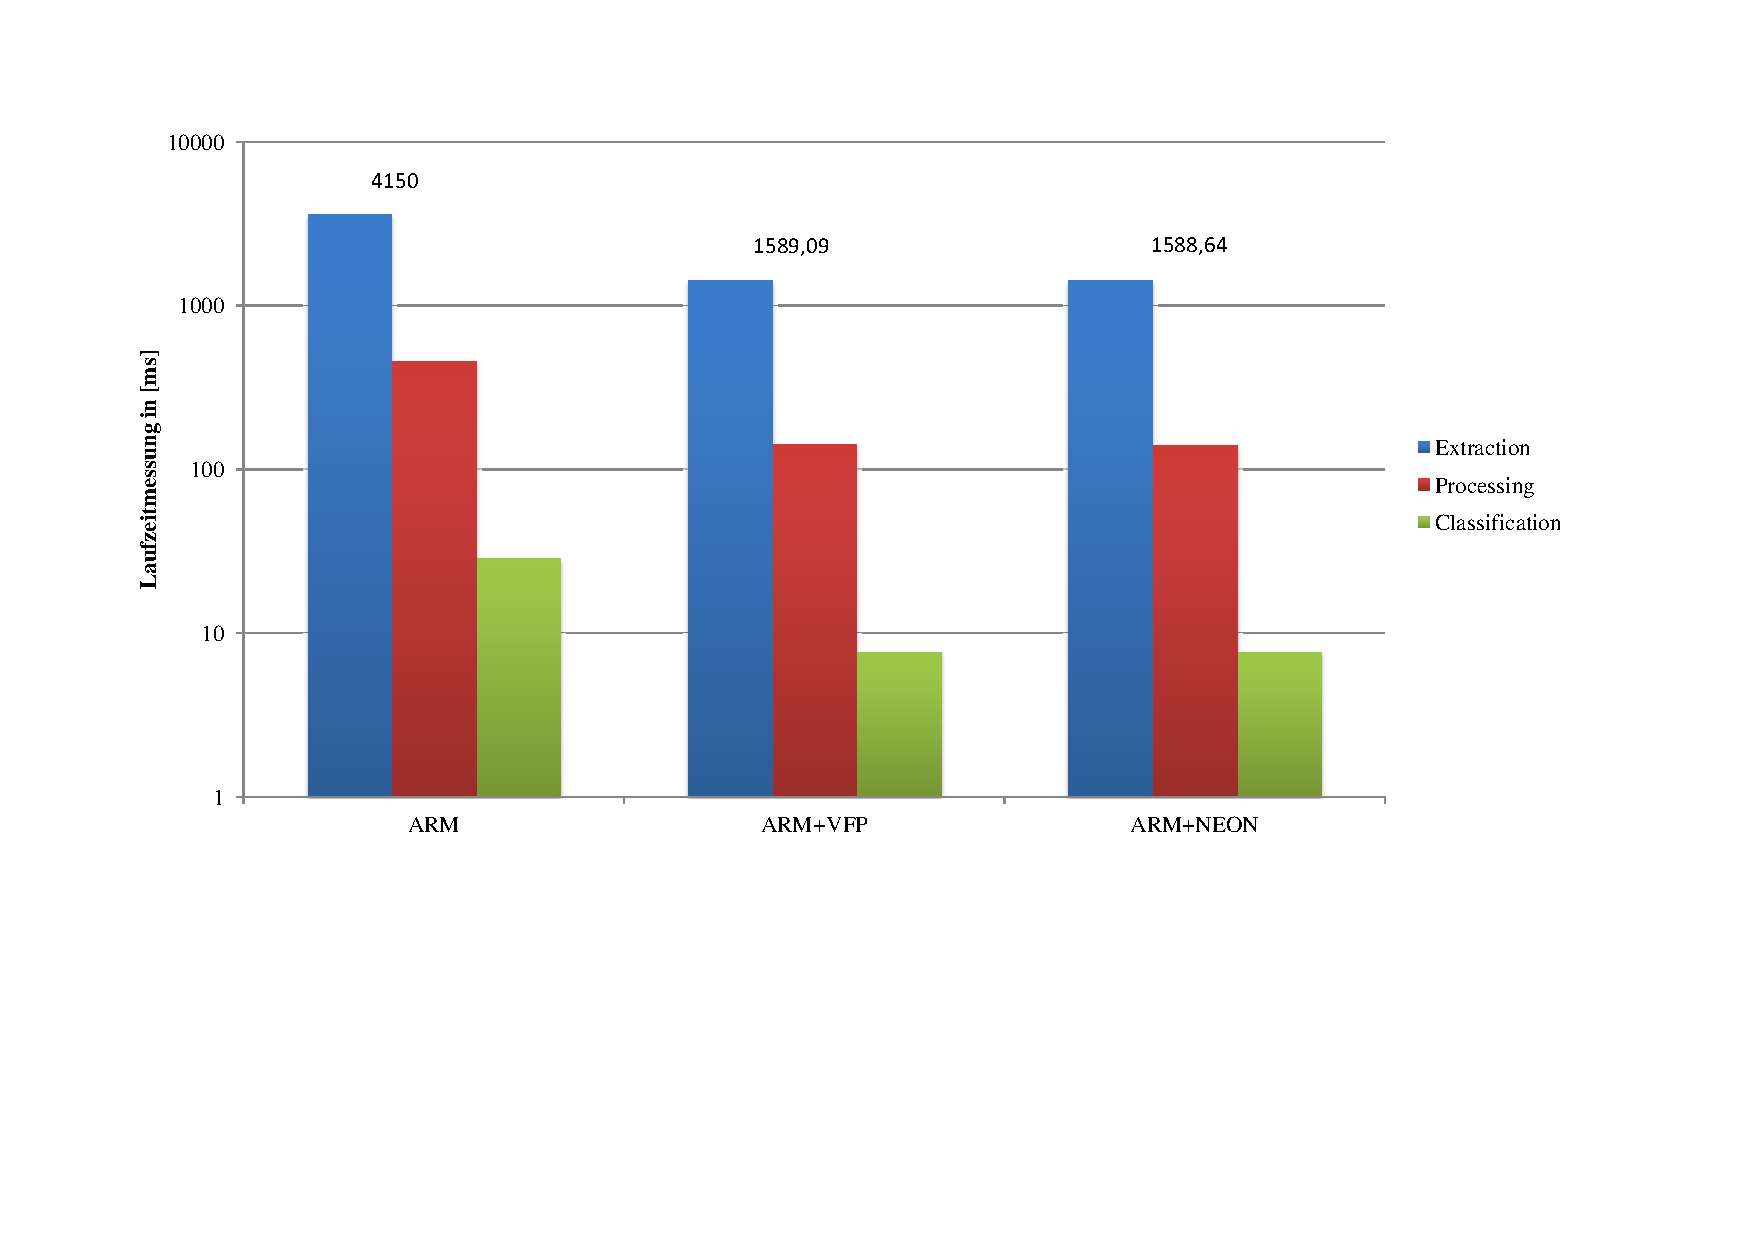
\includegraphics[width=1\textwidth]{../Pictures/fset2AVN.pdf}
	\caption{Laufzeiten in ms des Musikklassifikators f�r ARM, ARM+VFP und ARM+NEON am Beispiel des FeatureSets 2}
	\label{fig:armtime}
\end{figure} 
%
Aus \textbf{Abbildung \ref{fig:armtime}} lassen sich drei wesentliche Schl�sse ziehen:

\begin{enumerate}
\item Die Extraktionsphase hat in allen drei F�llen den gr��ten Anteil an der Laufzeit
\item Die reine ARM-Implementation hat die schlechteste Laufzeit
\item ARM+VFP und ARM+NEON scheinen gleichwertig zu sein
\end{enumerate}

Die Punkte 1 und 2 kann man so stehen lassen, da diese zu den erwarteten Ergebnissen z�hlen, aber Punkt 3 verwundert einen doch sehr. Wie kann es sein, dass trotz der in \textbf{Kapitel \ref{subsubsec:neon}} beschriebenen Vorteile der NEON-SIMD-Einheit gegen �ber der VFP-Einheit, beide Einheiten doch gleichwertig erscheinen? Es soll nochmals erw�hnt werden, dass beide Implementationen mit einer Compileroption f�r die jeweilige Floating Point-Einheit optimiert wurden. Ein Blick in den entstandenen Assemblercode der beiden Implementierungen gibt die Antwort auf die gestellte Frage. Hier finden sich in beiden F�llen nahezu gleiche Codes, das hei�t auch die NEON-SIMD-Einheit f�r nur die rein sklaren Operationen des VFP aus. Dieses erkl�rt einerseits, warum sich die Laufzeiten der beiden Implementationen nicht wesentlich voneinander unterscheiden und zeigt andererseits, dass es dem Compiler scheinbar nicht m�glich ist effektiv f�r die NEON-SIMD-Einheit optimierten Code zu generieren.\\\\
Da die Extraktionsphase sich als am zeitintensivsten herausgestellt hat, soll diese jetzt n�her analysiert werden.\\ 
Wie aus \textbf{Abbildung \ref{fig:1fset2}} zu entnehmen ist, fallt der gr��te Anteil der Laufzeit der Extraktionsphase mit knapp 60\% auf die Berechnung der FFT.
%
\begin{figure}[h]
	\centering
		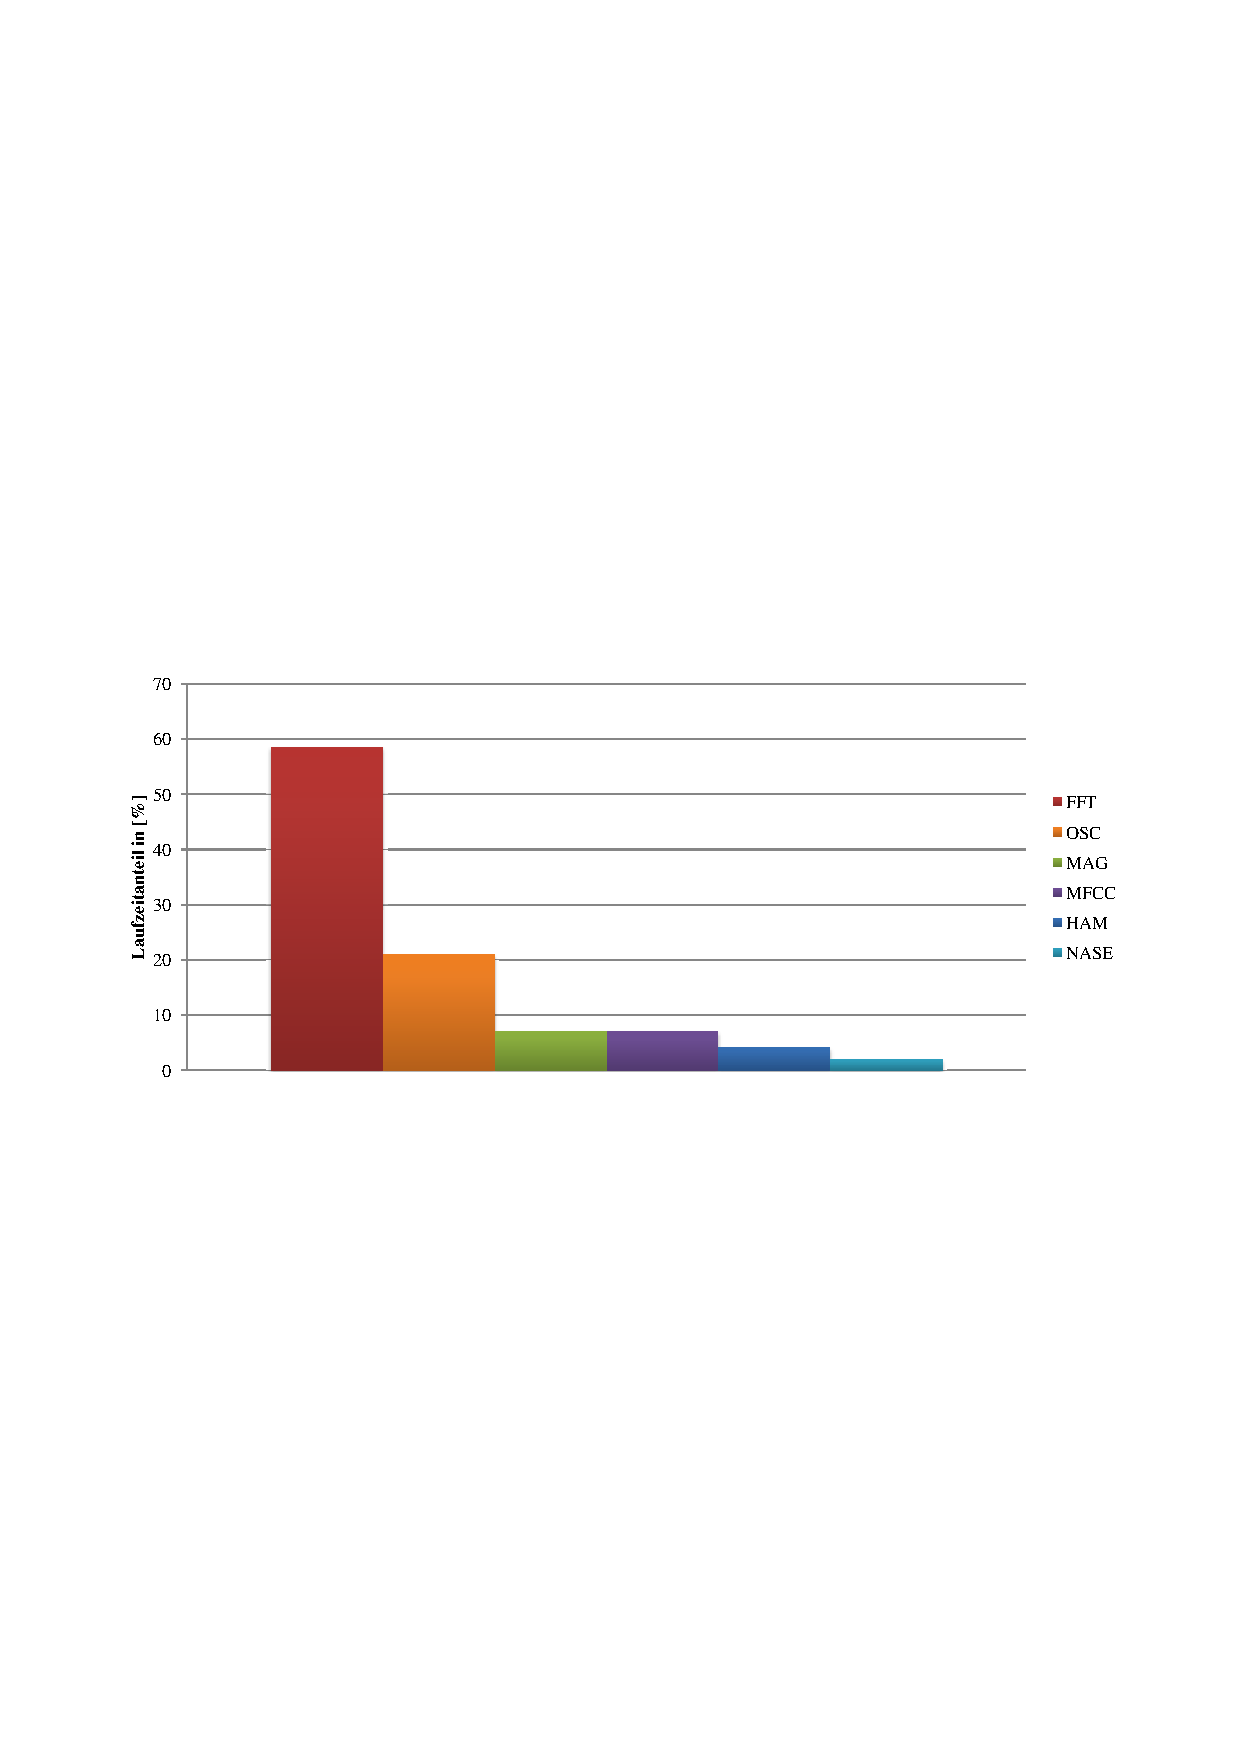
\includegraphics[width=1\textwidth]{../Pictures/1fset2.pdf}
	\caption{Detailliertere Laufzeitmessung der Extraktionsphase}
	\label{fig:1fset2}
\end{figure} 
%

\subsection{Libav als Optimierung der FFT}\label{subsec:optFFT}
\subsubsection{Laufzeitmessung}
\subsubsection{Aufbau der FFT}
\subsubsection{Einbindung}

\subsection{Optimierung der Amplitude of Spectrum}\label{subsec:optAOS}
\subsubsection{Laufzeitmessung}
\subsubsection{Codeanpassung}

\subsection{Optimierung von MFCC}

\subsection{Optimierung der Zero Crossing Rate}



 
